\chapter{Observing signal spectra of GNSS satellites}
In this chapter, we describe how SALSA can be utilized in observations of signals 
transmitted by GNSS satellites. Note that in this project we are currently able to investigate signals 
in a relative sense as an absolute flux density calibration of SALSA antennas has not been implemented yet.


\section{How does SALSA know where to point at ?}
Finding the location of GNSS satellites of interest on the sky can be tricky as they are in a continuous motion. The SALSA control 
program can however calculate the position of any GNSS satellite at any given time. It uses a so-called two-line element set 
(TLE) to localize an artificial Earth-orbiting object on the sky and be able to follow (track) it. 
TLE is a data format that encodes a list of orbital elements of an Earth-orbiting object for a given point in time.
As the name suggest, a trajectory of a target can be described using just two lines:
\begin{verbatim}
 1 29486U 06042A   16001.47634844 -.00000070  00000-0  00000+0 0  9996
 2 29486  55.7430 303.5601 0084444 331.9182 116.9546  2.00564670 67931
\end{verbatim}
With a sufficient prediction formula, the position and velocity of an object can be calculated, to some accuracy\footnote{The accuracy of TLE data is dependent upon few factors such as the target's orbit type or the amount 
of collected data. These factors usually vary for each generated element set, which, of course, affects our accuracy.}, at any point in the future or in the past. New element sets are generated with varying frequency, 
depending upon the object's orbit type. The interested reader is referred to \href{https://celestrak.com/}{CelesTrak} for more information on TLEs and an access to the TLE database.

\section{Tracking GNSS satellites}
In this subsection, we describe how to use SALSA interface to track GNSS satellites. For general introduction to the Graphical User Interface (GUI), the reader is referred to 
\emph{SALSA user manual} available at the \href{https://vale.oso.chalmers.se/salsa/support}{SALSA}  website. \par{}
Once we are familiar with the GUI of SALSA, one can start tracking GNSS satellites. In case SALSA telescopes (Vale/Brage) are started for the first time, it is necessary 
to reset the chosen telescope using the \verb!Reset! button located in the main window. This makes sure that the telescope tracks chosen objects correctly. \par{}
The module that allows us to cope with GNSS satellites is available after choosing \emph{GNSS} from the \emph{Desired} list in the main window of SALSA.
The GNSS-related part of the GUI consists of a combo box (in the main window) with a list of GNSS satellites available for tracking\footnote{This means satellites that are
above the local horizon.} and a separate window displaying current (calculated) positions of satellites on the sky. To track a satellite, choose one from the second combo box 
in the control program and press \verb!Track!. The telescope will start moving towards the chosen satellite. Note that it may take up some time 
to reach your desired position if you started pointing far away on the sky. Once the telescope reaches the desired position, the yellow color of the labels in the main window 
will disapear. This means that the telescope is now tracking the chosen satellite. To switch 
to a different satellite, click \verb!Stop!, choose a satellite from the list and click \verb!Track! again. The step-by-step 
demonstration for tracking a satellite is shown in Fig.~\ref{MainLab:GNSStracking}. \par{} 
It is also possible to observe at different angular separations relative to
the satellite that is being tracked. Conveniently, the SALSA control program can automatically track
positions relative to the chosen satellite by specifying local (altitude, azimuth) offsets. For example, if we are currently tracking a satellite and we want to 
point at the part of the sky that is always three degrees offset in azimuth from this satellite, click \verb!Stop!, enter an azimuth offset of 3 in one of the dedicated text 
boxes in the main window and press \verb!Track!. To switch to another relative position, you
have to first press \verb!Stop! to be able to input new offsets, and then \verb!Track! again to choose a new position. \par{}
\textbf{When you are done with your observations and would like to exit the program, choose \emph{Stow} as \emph{Desired}, press} \verb!Track! 
\textbf{to move the telescope into the stow position and wait until it reaches its destination.} This step puts telescopes in a save position that prevents them 
from being damaged while they are not used. 


\begin{figure}[ht] 
\centering
    \begin{subfigure}[a]{0.49\textwidth}
        \centering
        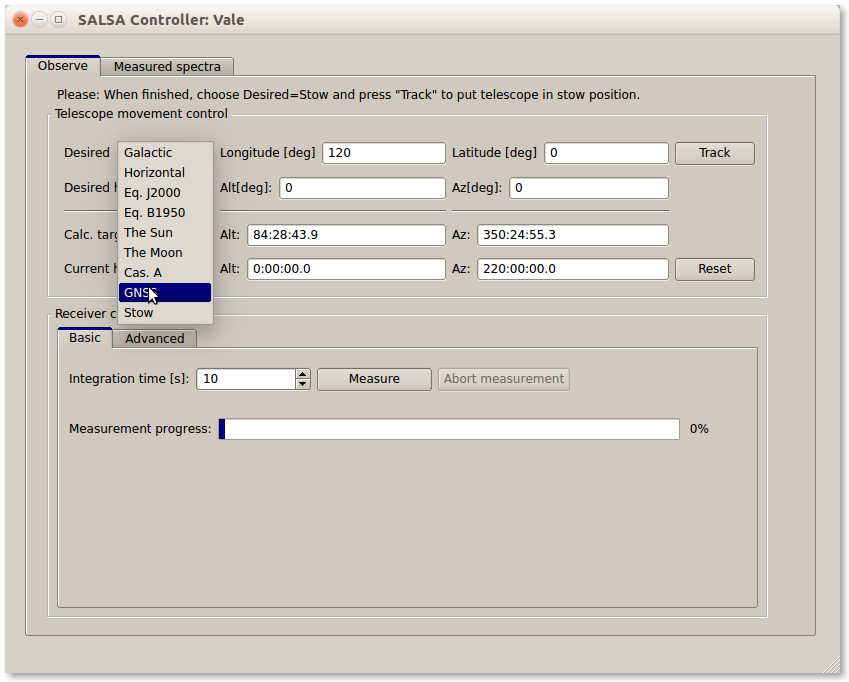
\includegraphics[width=1\columnwidth]{\plotFolder/GNSS_gui1.png}
        \caption{Choose \emph{GNSS} as \emph{Desired}.}
    \end{subfigure}%
    \begin{subfigure}[b]{0.49\textwidth}
        \centering
        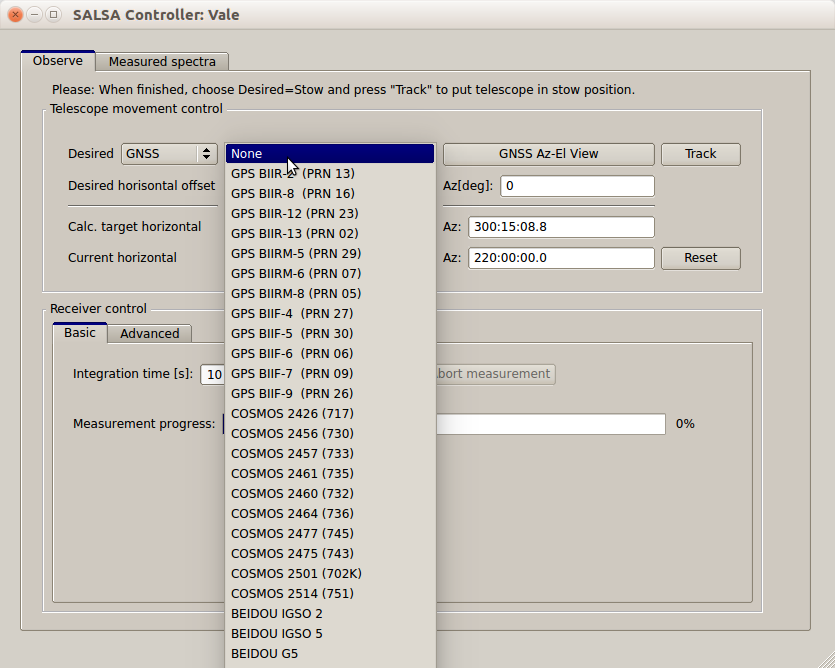
\includegraphics[width=1\columnwidth]{\plotFolder/GNSS_gui2.png}
        \caption{Choose a satellite from the list and click \emph{Track}.}
    \end{subfigure} \\
        \begin{subfigure}[a]{0.49\textwidth}
        \centering
        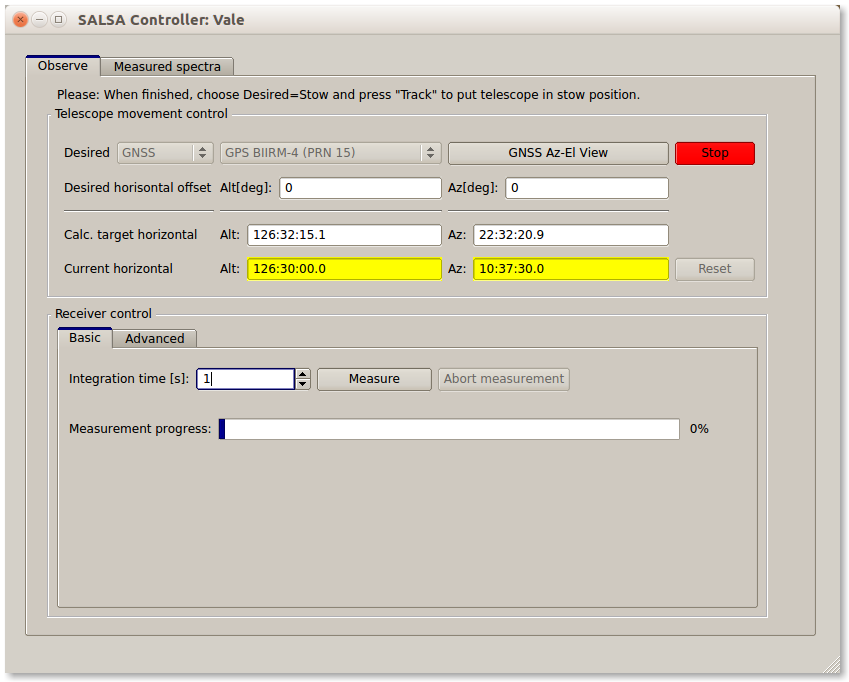
\includegraphics[width=1\columnwidth]{\plotFolder/GNSS_gui4.png}
        \caption{Telescope moves towards the chosen satellite.}
    \end{subfigure}%
    \begin{subfigure}[b]{0.49\textwidth}
        \centering
        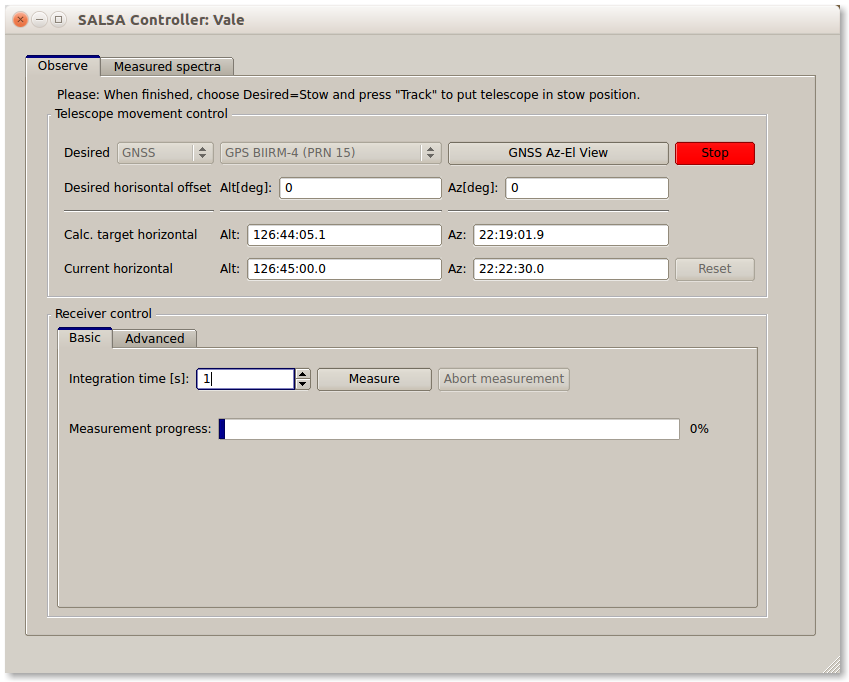
\includegraphics[width=1\columnwidth]{\plotFolder/GNSS_gui5.png}
        \caption{Telescope is tracking the object and SALSA is ready to measure.}
    \end{subfigure} 
  \caption{GNSS satellite tracking with SALSA.}    
\label{MainLab:GNSStracking}            

\end{figure} 

\section{Observing signals of GNSS satellites}
Once we are following the chosen GNSS satellite on the sky, one can start recording signals 
and investigating the obtained spectra\footnote{A plot of the radio emission as a function
of the frequency within a specific frequency range.}. To avoid obstacles or disturbing radio emission from the Earth, 
it is good to observe when the target GNSS satellite is as high above the horizon as possible. To find out
where the chosen satellite is currently on the local sky, you may use the Azimuth-Elevation window
available under the \verb!GNSS Az-El View! button~(Fig.~\ref{MainLab:AzElWindow}). The Altitude-Elevation (Az-El)
        coordinate system that is present there uses the observer's (telescope's) local horizon as the fundamental plane. In this system, the position of a target on the 
        sky is expressed in terms of the altitude (or elevation) and azimuth angles. The former (El) is the angle between the target and the observer's 
        local horizon. For visible objects it is an angle between 0 and 90 degrees. The latter (Az) is the angle of the object measured 
        around the horizon, with zero at north and increasing values towards the east (0--360 degrees).\par{}
\begin{figure}[t!] 
\centering
        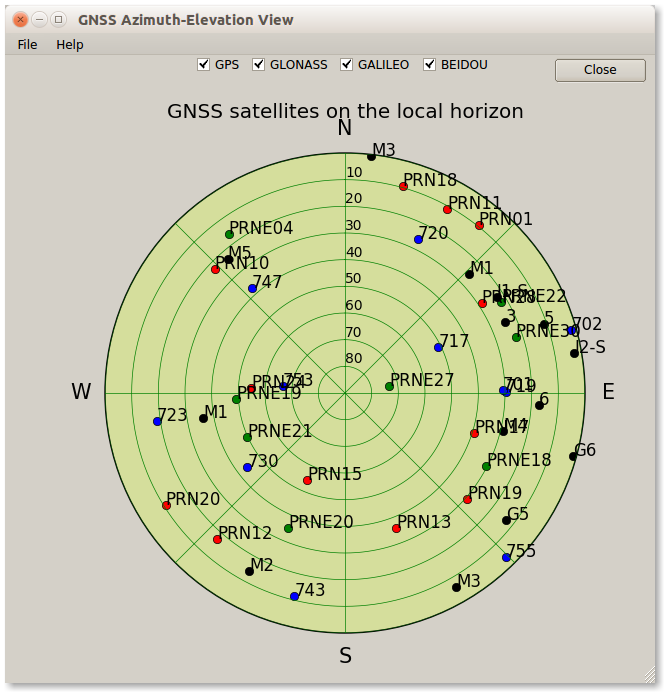
\includegraphics[width=0.65\textwidth]{\plotFolder/GNSS_gui3.png}
        \caption{Window with distribution of GNSS satellites on the local horizon. }
\label{MainLab:AzElWindow}            
\end{figure} 

The SALSA control program, as described in \emph{SALSA user manual}, was
developed to measure the radio emission from neutral hydrogen. In this case, it is crucial 
to find out how the emission changes with different frequencies close to 1420\,MHz. However, 
when observing signals transmitted by GNSS satellites, we are only interested in the total power 
received by the antenna in some frequency range (band). \par{}
Since SALSA's default observing frequency is 1420\,MHz, one needs to change it 
to one of the frequencies utilized by GNSS satellites~(See~Tab.\ref{tab:GNSSconstelations}). 
This is done on the \emph{Advanced} tab in the \emph{Receiver control} 
part of the control program. The default bandwidth does not need to be changed for this exercise, 
but 5~MHz can be set as the bandwidth that we would like to observe at. By default, the program 
will observe in the \emph{Switched} mode which is used for spectral line observations of hydrogen. 
Since we want only to look at the signal strength, we need to change this mode to
\emph{Signal}. This can be also done on the \emph{Advanced} tab in the \emph{Receiver control}
part. An example of the frequency/measurement setup for GNSS L1/E1 band is shown in Fig.~\ref{MainLab:fig:FrequencySetup}.\par{}
\begin{figure}[ht] 
\centering
        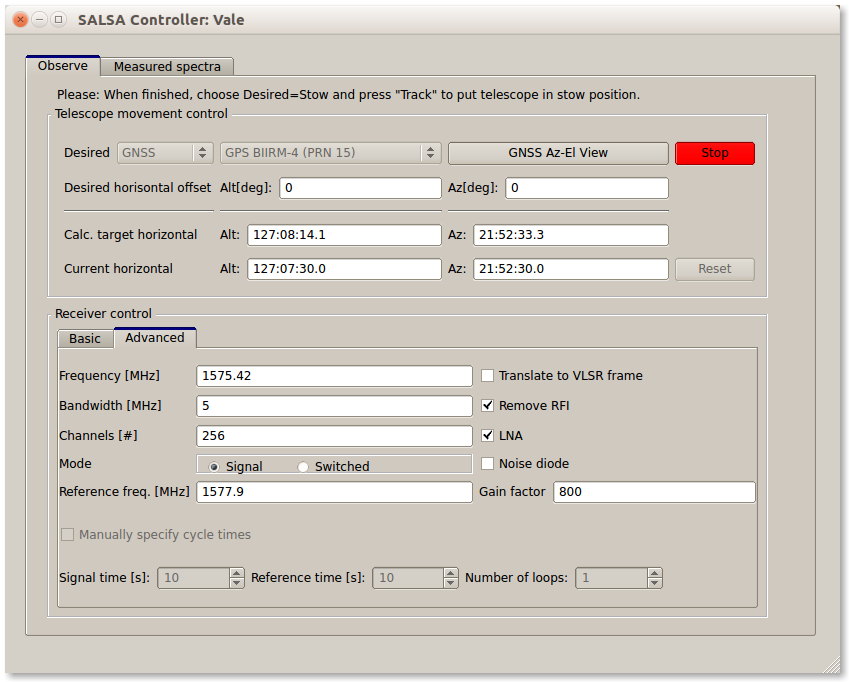
\includegraphics[width=0.65\textwidth]{\plotFolder/GNSS_gui6.png}
        \caption{Frequency and measurement setup for E1 / L1 band.}
\label{MainLab:fig:FrequencySetup}            
\end{figure} 
Once we have specified the frequency and the observing mode, we are ready to
measure. A default integration time of 10 seconds is enough to detect GNSS signals. 
The shorter observation time can be chosen on the \emph{Basic} tab in the \emph{Receiver control} 
part of the GUI. Make sure that you are tracking the satellite of interest and then press \verb!Measure!. 
The recorded spectrum will appear on the \emph{Measured spectra} tab. An example of the 
GPS signal spectrum obtained with SALSA is shown in Fig.~\ref{MainLab:fig:Spectrum}. 
In addition, the results can be displayed in the dB scale\footnote{For 100 K the result would be $10\cdot log_{10}(100K) = 20\,dBK$} 
and normalized by clicking the corresponding check boxes above the plot with the signal spectrum. \par{}

\begin{figure}[ht] 
\centering
        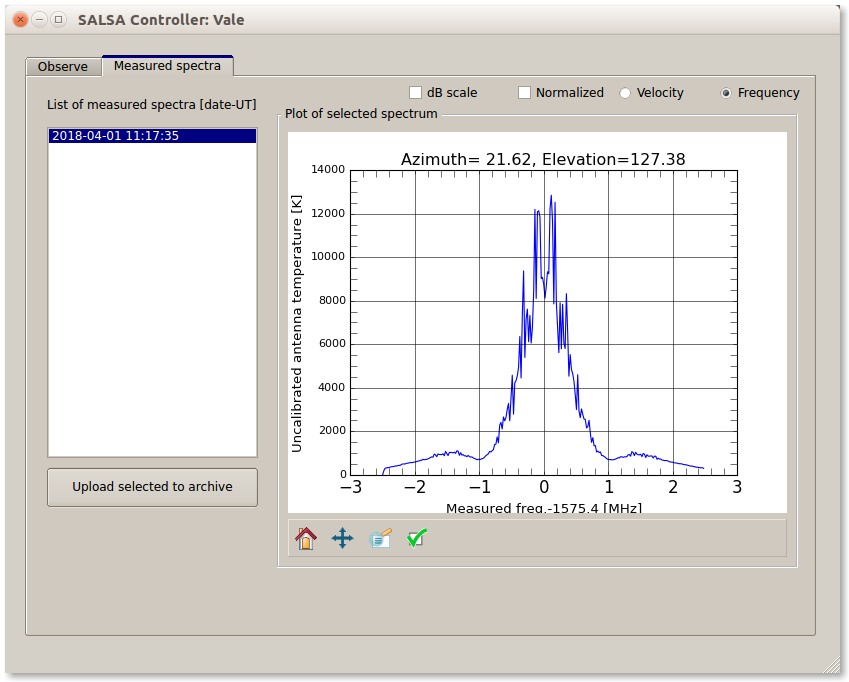
\includegraphics[width=0.85\textwidth]{\plotFolder/GNSS_gui7.png}
        \caption{Signal spectrum of PRN 15 (GPS) at L1 for the measurement time of one second. Note that the radio button in the upper right part of the
        window is set to \emph{Frequency}. }
\label{MainLab:fig:Spectrum}            
\end{figure} 
Currently, the measured signal strength is expressed as 'Uncalibrated antenna temperature [K] ' and can be interpreted only in a relative
sense, i.e. with respect to other radio sources (the Sun, ground noise, other satellites) as measuring the true signal strength with 
SALSA has not been implemented yet. \par{}

\section{Related questions}

\begin{itemize}
\item Can you name other applications of GNSS not mentioned in the following document ?
\item Each GPS satellite is visible at the same position on the sky every $11^h58^m2^s$. Asumming that the radius of the Earth is 6371 km, 
what is the orbital speed (in km/s) of GPS satellites\footnote{$v\approx 2\pi(R_{Earth}+a)/T$} ?
\item What is the free-space loss (in dB) for signals at L1-band and a distance of 25 000~km between a satellite and an observer ? What would 
happen to the free-space loss if we would like to use frequencies amounting to 10-12 GHz ?
\item Choose any GNSS satellite located close to the horizon and carry out observations. How does the spectrum look like ?
 \item The GPS L1 signal spectrum is shown in Fig.~\ref{MainLab:fig:Spectrum}. How does it look like for GALILEO satellites ?
 \item Choose any GLONASS satellite and measure the signal. Can you see the spectrum~? If not, why~?

\end{itemize}
